\documentclass{book}
\usepackage{tikz}
\usetikzlibrary{shadows}
\usetikzlibrary{decorations}
\usetikzlibrary{shapes.multipart}
\usetikzlibrary{shapes.symbols}

\newcommand{\InstructorNote}[1]{%
\marginpar{%
\parbox{.9in}{\begin{tikzpicture}
\node at (0,0) [double copy shadow={opacity=.5},tape,fill=blue!10,draw=blue,thick]
{\parbox{.75in}{\footnotesize {\sc Instructor Note}\\\texttt{#1}}};
\end{tikzpicture}}}
}

\newcommand{\FoodForThought}[1]{%
\marginpar{%
\parbox{.9in}{\begin{tikzpicture}
\node at (0,0) [double copy shadow={opacity=.5},tape,fill=blue!10,draw=blue,thick]
{\parbox{.75in}{\footnotesize {\sc Specialized}\\\texttt{#1}}};
\end{tikzpicture}}}
}
\begin{document}

Here's the macro I used in my book.  It's a marginpar, which may not be what we want, since things get dicey with two-sided documents.

\InstructorNote{For instructors only that is}

Goodbye

There are a large number of possibilities to try out.  In place of ``starburst'' in the above macro, try
\begin{enumerate}
\item cloud
\item starburst

\end{enumerate}


Other nice ones:
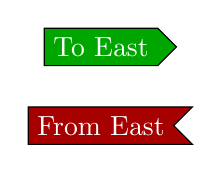
\begin{tikzpicture} [every node/.style={signal, draw, text=white, signal to=nowhere}] \node[fill=green!65!black, signal to=east] at (0,1) {To East}; \node[fill=red!65!black, signal from=east] at (0,0) {From East};
\end{tikzpicture}

It might make more sense to have these as the start of an environment, and not as margin notes.  Then we could have a little start and end symbol for the marked section of the environment.


\newpage
Here's the macro I used in my book.  It's a marginpar, which may not be what we want, since things get dicey with two-sided documents.

\FoodForThought{Some longish note here to see what happens.
Some longish note here to see what happens}

Goodbye

There are a large number of possibilities to try out.  In place of ``starburst'' in the above macro, try
\begin{enumerate}
\item cloud
\item starburst

\end{enumerate}


Other nice ones:
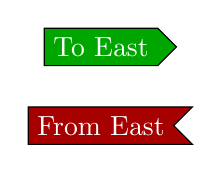
\begin{tikzpicture} [every node/.style={signal, draw, text=white, signal to=nowhere}] \node[fill=green!65!black, signal to=east] at (0,1) {To East}; \node[fill=red!65!black, signal from=east] at (0,0) {From East};
\end{tikzpicture}

It might make more sense to have these as the start of an environment, and not as margin notes.  Then we could have a little start and end symbol for the marked section of the environment.

\end{document}
